\documentclass{article}

% if you need to pass options to natbib, use, e.g.:
%     \PassOptionsToPackage{numbers, compress}{natbib}
% before loading neurips_2019

% ready for submission
% \usepackage{neurips_2019}

% to compile a preprint version, e.g., for submission to arXiv, add add the
% [preprint] option:
%     \usepackage[preprint]{neurips_2019}

% to compile a camera-ready version, add the [final] option, e.g.:
\usepackage[final]{neurips_2020}

% to avoid loading the natbib package, add option nonatbib:
%     \usepackage[nonatbib]{neurips_2019}

\usepackage[utf8]{inputenc} % allow utf-8 input
\usepackage[T1]{fontenc}    % use 8-bit T1 fonts
\usepackage{hyperref}       % hyperlinks
\usepackage{url}            % simple URL typesetting
\usepackage{booktabs}       % professional-quality tables
\usepackage{nicefrac}       % compact symbols for 1/2, etc.
\usepackage{microtype}      % microtypography
\usepackage{graphicx}
\usepackage{amsfonts}
\usepackage{amsmath}
\graphicspath{ {./assets/} }
\bibliographystyle{unsrtnat}



\title{Image Colorization using Deep Convolutional Networks and Generative Adversarial Networks}

% The \author macro works with any number of authors. There are two commands
% used to separate the names and addresses of multiple authors: \And and \AND.
%
% Using \And between authors leaves it to LaTeX to determine where to break the
% lines. Using \AND forces a line break at that point. So, if LaTeX puts 3 of 4
% authors names on the first line, and the last on the second line, try using
% \AND instead of \And before the third author name.

\author{%
  Anirudh Mukundan Raghavan\thanks{equal contribution}\\
  Department of Computer Science\\
  University of Florida\\
  \texttt{araghavan@ufl.edu} \\
  \And
  Prajwal Dondiganahalli Prakash\thanks{equal contribution.}\\
  Department of Computer Science\\
  University of Florida\\
  \texttt{prajwal.dondigan@ufl.edu} \\
}

\begin{document}

\maketitle

\begin{abstract}
  In this project, we address the problem of automatically generating a
  plausible colored photograph given a grayscale image using Convolutional
  Neural Networks. We explore two methods - conventional supervised machine
  learning and generative modeling using Generative Adversarial Networks. In the
  first method, we frame the problem as an optimization problem to generate a
  mapping between the pixels in the input grayscale scale and the target color
  image. In the second method, we use a generator-discriminator model pair that
  is adversarially trained so that the generator produces outputs
  indistinguishable from the actual color images. We explore several
  architectures/models and loss functions to obtain the most aesthetically
  pleasing colored images. We also discuss state-of-the-art enhancements to our
  two models that could improve their performances. We provide a quantitative
  analysis of our results and discuss areas for further research.
\end{abstract}

\section{Introduction}

\subsection{Background}

Image colorization is a fascinating topic to study in deep learning. It involves
computer vision techniques, such as image classification, and image segmentation
working together. Traditionally, to colorize an image, a model must first
classify the various objects present in the image. Next, the model must locate
the object in the image. Last, the model must apply the correct color to all the
objects present in the image. One might think that there are too many choices
for color, a shirt may be of any color or shade in the RGB spectrum, a wall may
be painted in any color and a car may have any paint job. Thus, our problem is
multimodal, where we may have multiple valid predictions for a single image.
This is partially true - while there exist many choices for common objects, most
objects have a specific choice of colors. For example, the sky is either blue or
black depending on the time of day, the sun is always yellow, the moon is always
white, etc. A common problem faced while training models is the lack of data.
This is not a problem for this task, as we can simply convert existing images to
grayscale and pair them with their color versions to train the network. Thus,
predicting color is more tractable than we think, especially using Deep
Learning.

Two popular methods exist to colorize grayscale images using machine learning –
user-guided, and automatic colorization. In the first method, a human provides
additional semantic input, usually by drawing strokes over the grayscale image,
providing hints to the model. This method has historically provided accurate
results but requires intensive user interaction. The second model works either
by matching a picture to its colored version and learning parametric mappings
from grayscale to color from large-scale image data. This is the method we will
be using to build our model.

We will use a Convolutional Neural Network and a Generative Adversarial Network
to colorize images and then compare the results from both networks.

\subsection{Problem Statement}

Image colorization is a translation problem, where we try to map the input image
to an output image, where the images are represented as high dimensional arrays
of numbers. It can be seen as a regression problem on individual pixels, where
we try to predict the values of each pixel in the output based on the pixel
value in the input. Our network will try to generate an output but with
different values for the pixels.

Assuming each input image $\mathbf{X}$ has the dimensions $h * w$, and is
encoded in a 3-channel colorspace (e.g. RGB colorspace), then $\mathbf{X} \in
\mathrm{R}^{\mathit{h * w * 3}}$. $\mathbf{\Phi} \in \mathrm{R}^{\mathit{H * W *
3}}$ is a pixel-to-pixel transformation (e.g. normalization) on $\mathbf{X}$.
$\mathbf{Y} \in \mathrm{R}^{\mathit{h * w * 3}}$ is the target output image in
the dataset and $\mathbf{\widehat{Y}} \in \mathrm{R}^{\mathit{h * w * 3}}$ is
the image generated from our model.

\begin{equation}
  \mathbf{\widehat{Y}}
  =
  \mathop{f} (\mathbf{\Phi})
\end{equation}

\begin{equation} \label{eq:1}
  \mathop{minimise}
  \mathrm{L} (\mathbf{Y}, \mathbf{\widehat{Y}})
  =
  \sum_{h, w} l (y_{h, w}, \widehat{y}_{h, w})
\end{equation}

Our primary objective is then defined by equation \ref{eq:1}, where
$\mathop{l}$ is a function that defines the distance between two pixel values.

Since there are very few constraints for the values the pixels can take, there
are no right or wrong values for the pixels. Each image can be colored in
multiple ways. This leads to an interesting challenge, where we experiment with
different loss functions and network architectures to see which one gives us
aesthetically pleasing images.

\subsection{Algorithms}

\subsubsection{Convolutional Neural Networks}

A Convolutional Neural Network (CNN) is a neural network, i.e., it is made up of
layers of perceptrons that are connected to each other through connections with
learnable weights. Each of these perceptrons receive an input and computes a dot
product with its weights. Optionally, it may apply a non-linear function to the
output. The difference in a CNN is that the layers typically are built to deal
with high-dimensional data, such as images, where filters need to be learned to
extract features from specific parts of the high-dimensional data. They are
composed of the following layers:

\subsubsection{Convolutional Layer}

A convolutional layer

\begin{itemize}
  \item Accepts a volume of size $\mathbf{W}_1 * \mathbf{H}_1 * \mathbf{D}_1$
  \item Requires four hyperparameters: number of filters
  $K$, their spatial extent $F$, the stride $S$, the amount of zero padding $P$.
  \item Produces a volume of size $\mathbf{W}_2 * \mathbf{H}_2 * \mathbf{D}_2$ where:
\end{itemize}

\begin{eqnarray} \nonumber
  \mathbf{W}_2 & = & \frac{\mathbf{W}_1 - F + 2P}{S + 1} \\ \nonumber
  \mathbf{H}_2 & = & \frac{\mathbf{H}_2 - F + 2P}{S + 1} \\ \nonumber
  \mathbf{D}_2 & = & K \nonumber
\end{eqnarray}

In the output volume, the d-th depth slice (of size $\mathbf{W}_2 *
\mathbf{H}_2$) is the result of performing a valid convolution of the $d$-th
filter over the input volume with a stride of S, and then offset by $d$-th bias.

\subsubsection{Pooling Layer}

The function of the pooling layer is to reduce the size of the output of a convolutional layer, to
reduce the number of parameters in the network. This reduces the amount of computation required to
train the network. It also helps in controlling overfitting. The most common pooling layer is with
filters of size 2*2.

\begin{itemize}
  \item Accept a volume of size $\mathbf{W}_1 * \mathbf{H}_1 * \mathbf{D}_1$
  \item Requires two hyperparameters: their spatial extent $F$, the stride $S$
  \item Produces a volume of size $\mathbf{W}_2 * \mathbf{H}_2 * \mathbf{D}_2$.
\end{itemize}

\begin{eqnarray} \nonumber
  \mathbf{W}_2 & = & \frac{\mathbf{W}_1 - F}{S + 1} \\ \nonumber
  \mathbf{H}_2 & = & \frac{\mathbf{H}_1 - F}{S + 1} \\ \nonumber
  \mathbf{D}_2 & = & \mathbf{D1} \nonumber
\end{eqnarray}

\subsubsection{Fully Connected Layer}
The neurons in this layer are connected to all the activations of the previous
layer i.e. they maintain the shape of the previous layer. These layers are
similar to the ones used in ordinary neural networks. They accept an input x,
compute a matrix multiplication with their weights, and add a bias. Additionally,
they can also apply a non-linearity such as ReLU, sigmoid to the output.

\subsubsection{Generative Adversarial Networks}

Generative models are unsupervised learning models that model the patterns and
irregularities in the input data and can generate new examples that are
indistinguishable from the ones in the input data. A Generative Adversarial
Network (GAN) is a method to train such generative models by pairing them with a
discriminative model. Hence, a GAN has two sub-models, a generator model that
generates new examples, and a discriminator model that classifies whether the
examples are real (from the input data) or generated by the generator model. The
two sub-models are trained together in a zero-sum game until the generator model
can fool the discriminator model about half the time, implying that the
generator model generates examples that are almost indistinguishable from the
(real) ones in the input data. The term adversarial implies that the model
rewards conflict between the generator model and the discriminator model. There
are many applications of such generator-discriminator networks, including
generating photorealistic images of people, objects, or scenes.

\section{Dataset}

We used the CIFAR-10 dataset to train both our models. The images in this
dataset have the dimensions 32x32 and is encoded in the RGB colorspace. While
these dimensions do not translate to a model that could be used to colorize
real-world images, the small dimensions allowed us to deal with memory and
computation constraints. We did not focus on a specific category and instead
trained our models on all the 50,000 images in the training set to build a
more generalized model.

\subsection{Preprocessing}

The 32x32x3 images in the RGB colorspace were converted into the CIE L*a*b
colorspace. The \textit{l} (luminance) channel is sufficient to represent the
grayscale image and the all the color information is encoded into the \textit{a}
and \textit{b} channels. Thus we could generate a dataset with input dimensions
32x32x1, and output dimensions 32x32x2 instead of dealing with 32x32x3 images as
the input and output images. To get the final image from the output, the \textit{l}
channel is concatenated with the \textit{a} and \textit{b} and converted back to
the RGB colorspace.

\section{Implementation}

\subsection{Convolutional Neural Networks}

We frame the problem as a regression problem - given an input lightness channel
$\mathbf{X} \in \mathbb{R}^{HxWx1}$, our objective is to learn a mapping
$\mathbf{\widehat{Y}} = f(\mathbf{X})$ to the two associated color channels
$\mathbf{Y} \in \mathbb{R}^{HxWx2}$.

\begin{equation}
  \mathrm{L}_2(\mathbf{Y}, \mathbf{\widehat{Y}})
  =
  \frac{1}{2} || \mathbf{Y} - \mathbf{\widehat{Y}} ||^2_2
  =
  \frac{1}{2} \sum_{h, w} (y_{h, w} - \hat{y}_{h, w})^2
\end{equation}

\subsubsection{Network Architecture}

We used the architecture as described in figure \ref{fig:cnn-mse}. Each
convolution layer uses \textit{ReLU} as the activation function. Experimenting
with \textit{tanh} as the activation function for just the final convolution
layer gave us better results. We used a stride length of 2x2 in the 1st, 4th and
6th convolution layers, while left it at 1x1 for the remaining layers.

\begin{figure}[h]
  \centering
  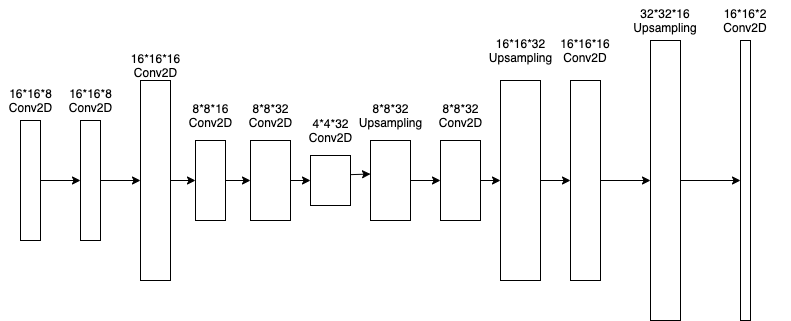
\includegraphics[width=\textwidth]{CNN-MSE-model.png}
  \caption{Model of the Convolutional Neural Network}
  \label{fig:cnn-mse}
  \centering
\end{figure}

\subsubsection{Training}
We used stochastic gradient descent to train the network, with the mean squared
error loss function. We start with a learning rate of 1e-2. When the loss
plateaus and stays the same for more than two iterations, we decrease the
learning rate by a factor of 2e-2. We trained our model for 50 epochs.

\subsection{Generative Adversarial Networks}

Typically, the input to the generator model is pseudorandomly produced noise. In
our scenario, the input to the generator is the grayscale image, and the output
we'd like it to generate is a colorized version of the grayscale image. Since an
additional input is provided (instead of a latent noise vector), our model is a
conditional GAN. In effect, we'd like the network to learn a transformation from
the input image to a target image. Our implementation is loosely based on the
Pix2Pix conditional GAN model. Here, the generator applies some function (that
is learned via training) to the input grayscale image producing an image that is
intended to be the colorized version of the input image. The discriminator
compares this output image and the corresponding color image (the ground truth)
from the dataset and attempts to classify the image as real or generated.

In the Pix2Pix model, \cite{DBLP:journals/corr/IsolaZZE16} use a 3-channel input
to both, the generator, and the discriminator, producing a 3-channel output. We
use the CIELAB color space to represent images in our implementation, where 1
channel is enough to represent the grayscale image, and 2 channels are enough to
represent all the color information.

\subsubsection{Generator Architecture}

The generator model in our implementation follows the encoder-decoder pattern as
in the figure. The input is a grayscale 32-by-32-pixel image represented by the
\textit{l}-channel of the CIE L*a*b* colorspace. The output is a 32-by-32-pixel
image represented by the a and b channels of the CIE L*a*b* colorspace. The
encoder layers of the generator downsample the input image with a series of
encoders into a much smaller higher-level representation of the image features.
Each encoder comprises of a convolutional layer, followed by a batch
normalization layer and an activation function. The decoder stack upsamples this
high-level feature representation and reverse the action of the encoder layers.
Each decoder comprises of a deconvolution (the transpose of a convolution
operation), followed by batch normalization and an activation function. The
activation function used in the encoder in \textit{Leaky ReLU}. Batch
normalization is applied to the transposed convolution in the decoder followed
by dropout (for the first three blocks). The activation function used in the
decoder blocks is \textit{ReLU}.

While the implementation of the generator in the Pix2Pix model uses a U-Net
instead of a conventional stack of encoders and decoders, our implementation
imitates the same behavior with the use of "skip connections" which directly
connect upsampling layers to downsampling layers as in the figure. This
effectively gives the network the option of skipping an upsampling
layer-downsampling layer pair if it doesn't have a use for it.

\begin{figure}[h]
  \centering
  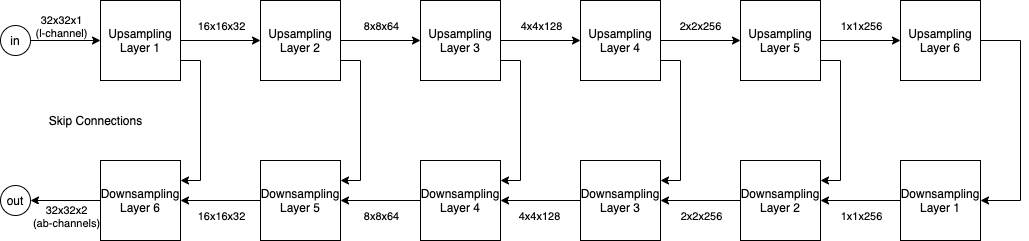
\includegraphics[width=\textwidth]{Generator1.png}
  \caption{Architecture of the Generator}
  \label{fig:generator-architecture}
  \centering
\end{figure}

\subsubsection{Generator Hyperparameters and Loss}

The generator loss is based on sigmoid cross entropy of the generated images
and and array of ones. \cite{DBLP:journals/corr/IsolaZZE16} also include a L1
loss which is the mean absolute error between the generated image and the target
image. We use the same generator loss function as described by
\cite{DBLP:journals/corr/IsolaZZE16}, which is defined in equation \ref{eqn:gan-loss}

\begin{equation} \label{eqn:gan-loss}
  \text{Generator Loss} = \text{sigmoid-loss} + \lambda * \text{L1-loss}
\end{equation}

The optimizer function used was Adam, which is based on stochastic gradient
descent. The learning rate was set to 2e-4, and the exponential decay rates for
the first moment estimates was set to 0.5. $\lambda$ was set to 100 as in the
paper.

\subsubsection{Discriminator Architecture}

The discriminator in the original Pix2Pix model is a PatchGAN. In our
implementation, the discriminator is a more conventional classifier as shown in
figure \ref{fig:discriminator-model}. It takes in the \textit{l}-channel from
the input data stacked with the \textit{ab} channels from the generator output
or the input data. It returns the probability of the image being generated by
the generator.

\begin{figure}[h]
  \centering
  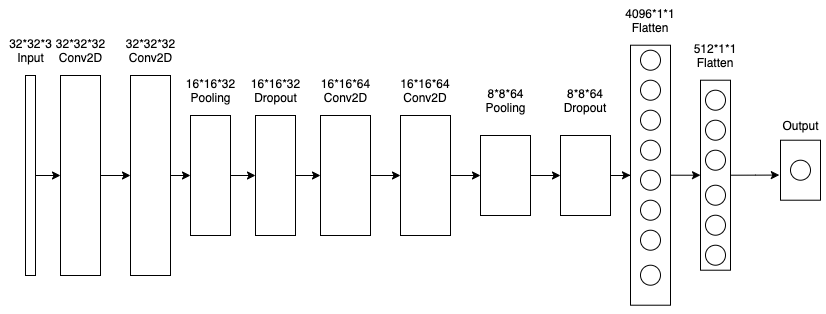
\includegraphics[width=\textwidth]{Discriminator.png}
  \caption{The Discriminator Model}
  \label{fig:discriminator-model}
  \centering
\end{figure}

\subsubsection{Discriminator Hyperparameters and Loss}

The total discriminator loss is the sum of two components - a real loss
component which is the sigmoid cross-entropy loss of the real images
(\textit{lab} from the input dataset) and an array of ones, and a generated loss
which is the sigmoid cross-entropy loss of the generated images (\textit{l} from
the input dataset concatenated with the \textit{ab} output from the generator)
and an array of zeros.

The optimizer function used was Adam, which is based on stochastic gradient
descent. The learning rate was set to 2e-4, and the exponential decay rates for
the first moment estimates were set to 0.5.

\subsubsection{Training}

Our implementation trains the discriminator model and the generator model in two
alternating steps. This process is illustrated in figure \ref{fig:training}.

\begin{itemize}
  \item The generator produces an initial output image from the input grayscale image.
  \item The discrimator classifies this generated output by concatenating it with the input and comparing it with the target concatenated with the input.
  \item The parameters of the discriminator are updated through the discriminator optimizer function based on the classification error.
  \item The parameters of the generator are also adjusted through the generator optimizer function based on the classification error by the discriminator.
\end{itemize}

We performed the training for about 350 epochs, and the metrics of the models
still seemed to improve with further epochs. Thus giving the model some more
epochs should further improve its performance.

\begin{figure}[h]
  \centering
  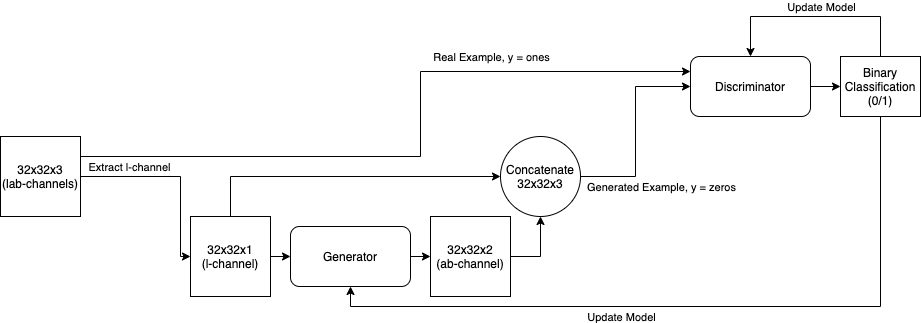
\includegraphics[width=\textwidth]{Training.png}
  \caption{The Training Process}
  \label{fig:training}
  \centering
\end{figure}

\section{Results}

\begin{table}[h!]
  \caption{Results - Successful original image replications by both models}
  \label{tab:1}
  \centering
  \begin{tabular}{ccccc}
    \toprule
    Grayscale Image & Ground Truth & CNN (ReLU) & CNN (tanh) & cGAN \\
    \midrule
    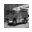
\includegraphics[width=2cm]{results3/23-bw.png} & 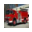
\includegraphics[width=2cm]{results3/23-gt.png} & 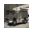
\includegraphics[width=2cm]{results5/23-relucnn.png} & 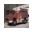
\includegraphics[width=2cm]{results5/23-tanhcnn.png} & 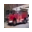
\includegraphics[width=2cm]{results3/23-gan.png} \\
    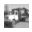
\includegraphics[width=2cm]{results3/45-bw.png} & 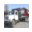
\includegraphics[width=2cm]{results3/45-gt.png} & 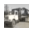
\includegraphics[width=2cm]{results5/45-relucnn.png} & 
\includegraphics[width=2cm]{results5/45-tanhcnn.png} & 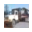
\includegraphics[width=2cm]{results3/45-gan.png} \\
    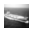
\includegraphics[width=2cm]{results3/54-bw.png} & 
\includegraphics[width=2cm]{results3/54-gt.png} & 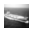
\includegraphics[width=2cm]{results5/54-relucnn.png} & 
\includegraphics[width=2cm]{results5/54-tanhcnn.png} & 
\includegraphics[width=2cm]{results3/54-gan.png} \\
    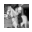
\includegraphics[width=2cm]{results3/56-bw.png} & 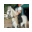
\includegraphics[width=2cm]{results3/56-gt.png} & 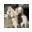
\includegraphics[width=2cm]{results5/56-relucnn.png} & 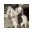
\includegraphics[width=2cm]{results5/56-tanhcnn.png} & 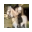
\includegraphics[width=2cm]{results3/56-gan.png} \\
    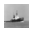
\includegraphics[width=2cm]{results3/72-bw.png} & 
\includegraphics[width=2cm]{results3/72-gt.png} & 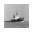
\includegraphics[width=2cm]{results5/72-relucnn.png} & 
\includegraphics[width=2cm]{results5/72-tanhcnn.png} & 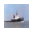
\includegraphics[width=2cm]{results3/72-gan.png} \\
    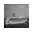
\includegraphics[width=2cm]{results3/73-bw.png} & 
\includegraphics[width=2cm]{results3/73-gt.png} & 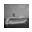
\includegraphics[width=2cm]{results5/73-relucnn.png} & 
\includegraphics[width=2cm]{results5/73-tanhcnn.png} & 
\includegraphics[width=2cm]{results3/73-gan.png} \\
    \bottomrule
  \end{tabular}
\end{table}

\begin{table}[h!]
  \caption{Results - Successful original image replications by the GAN}
  \label{tab:2}
  \centering
  \begin{tabular}{ccccc}
    \toprule
    Grayscale Image & Ground Truth & CNN (ReLU) & CNN (tanh) & cGAN \\
    \midrule
    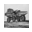
\includegraphics[width=2cm]{results3/171-bw.png} & 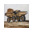
\includegraphics[width=2cm]{results3/171-gt.png} & 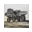
\includegraphics[width=2cm]{results5/171-relucnn.png} & 
\includegraphics[width=2cm]{results5/171-tanhcnn.png} & 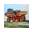
\includegraphics[width=2cm]{results3/171-gan.png} \\
    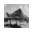
\includegraphics[width=2cm]{results3/179-bw.png} & 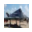
\includegraphics[width=2cm]{results3/179-gt.png} & 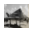
\includegraphics[width=2cm]{results5/179-relucnn.png} & 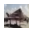
\includegraphics[width=2cm]{results5/179-tanhcnn.png} & 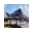
\includegraphics[width=2cm]{results3/179-gan.png} \\
    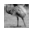
\includegraphics[width=2cm]{results3/219-bw.png} & 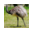
\includegraphics[width=2cm]{results3/219-gt.png} & 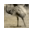
\includegraphics[width=2cm]{results5/219-relucnn.png} & 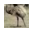
\includegraphics[width=2cm]{results5/219-tanhcnn.png} & 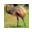
\includegraphics[width=2cm]{results3/219-gan.png} \\
    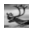
\includegraphics[width=2cm]{results3/40-bw.png} & \includegraphics[width=2cm]{results3/40-gt.png} & \includegraphics[width=2cm]{results5/40-relucnn.png} & \includegraphics[width=2cm]{results5/40-tanhcnn.png} & \includegraphics[width=2cm]{results3/40-gan.png} \\
    \bottomrule
  \end{tabular}
\end{table}

\begin{table}[h!]
  \caption{Results - Realistic Colorizations, not necessarily similar to the input image}
  \label{tab:3}
  \centering
  \begin{tabular}{ccccc}
    \toprule
    Grayscale Image & Ground Truth & CNN (ReLU) & CNN (tanh) & cGAN \\
    \midrule
    \includegraphics[width=2cm]{results3/83-bw.png} & \includegraphics[width=2cm]{results3/83-gt.png} & \includegraphics[width=2cm]{results5/83-relucnn.png} & \includegraphics[width=2cm]{results5/83-tanhcnn.png} & \includegraphics[width=2cm]{results3/83-gan.png} \\
    \includegraphics[width=2cm]{results3/97-bw.png} & \includegraphics[width=2cm]{results3/97-gt.png} & \includegraphics[width=2cm]{results5/97-relucnn.png} & \includegraphics[width=2cm]{results5/97-tanhcnn.png} & \includegraphics[width=2cm]{results3/97-gan.png} \\
    \includegraphics[width=2cm]{results3/192-bw.png} & \includegraphics[width=2cm]{results3/192-gt.png} & \includegraphics[width=2cm]{results5/192-relucnn.png} & \includegraphics[width=2cm]{results5/192-tanhcnn.png} & \includegraphics[width=2cm]{results3/192-gan.png} \\
    \bottomrule
  \end{tabular}
\end{table}

\begin{table}[h!]
  \caption{Results - Failed Samples}
  \label{tab:4}
  \centering
  \begin{tabular}{ccccc}
    \toprule
    Grayscale Image & Ground Truth & CNN - ReLU & CNN - tanh & cGAN \\
    \midrule
    \includegraphics[width=2cm]{results3/133-bw.png} & \includegraphics[width=2cm]{results3/133-gt.png} & \includegraphics[width=2cm]{results5/133-relucnn.png} & \includegraphics[width=2cm]{results5/133-tanhcnn.png} & \includegraphics[width=2cm]{results3/133-gan.png} \\
    \includegraphics[width=2cm]{results3/81-bw.png} & \includegraphics[width=2cm]{results3/81-gt.png} & \includegraphics[width=2cm]{results5/81-relucnn.png} & \includegraphics[width=2cm]{results5/81-tanhcnn.png} & \includegraphics[width=2cm]{results3/81-gan.png} \\
    \includegraphics[width=2cm]{results3/123-bw.png} & \includegraphics[width=2cm]{results3/123-gt.png} & \includegraphics[width=2cm]{results5/123-relucnn.png} & \includegraphics[width=2cm]{results5/123-tanhcnn.png} & \includegraphics[width=2cm]{results3/123-gan.png} \\
    \includegraphics[width=2cm]{results3/246-bw.png} & \includegraphics[width=2cm]{results3/246-gt.png} & \includegraphics[width=2cm]{results5/246-relucnn.png} & \includegraphics[width=2cm]{results5/246-tanhcnn.png} & \includegraphics[width=2cm]{results3/246-gan.png} \\
    \bottomrule
  \end{tabular}
\end{table}

The results of our models on some of the samples from the training set are in tables
\ref{tab:1}, \ref{tab:2}, and \ref{tab:3}, \ref{tab:4}. Table \ref{tab:1} displays the
images, whose colorized versions were able to be replicated closely by all our
models. Table \ref{tab:2} displays the images, where the GAN model was able to perform
better on. Table \ref{tab:3} displays some images which do not match the ground-truth
images but are realistic nevertheless. Table \ref{tab:4} displays the images which all
our implementations performed poorly on.

It is clear from the results that our GAN implementation performs the best
consistently over all the samples in the test set. The L2 loss regression also
performs well, except for the sepia tones that result from the same pattern
(e.g. a car) taking on multiple colors in the ground-truth images causing
averaging. It can also be seen that using the \textit{tanh} activation function
generates better results than the \textit{ReLU} activation function.

\subsection{Quantitative Metrics}

\cite{agrawalexploring} use the idea of closeness as a rough measure of accuracy
and acknowledge that it may not be a good metric to measure our models due to the
objective nature of the problem.

\section{Conclusion and Future Work}

Based on our experiments, we find that convolutional neural networks can be used
to colorize images to an acceptable degree of realism. However, there are
several enhancements that we could make to both our implementations.

\subsection{Classification Instead of Regression}

\cite{Nazeri_2018} conclude that while L2 loss can work well, it often leads to
desaturated sepia tones in the output images, as observed by us. The problem can
be reframed as a classification problem where the \textit{a} and \textit{b}
space can be quantised into bins. \cite{Nazeri_2018} use 10 bins corresponding
to a range of 20 pixels (the \textit{a} and \textit{b} channels have values from
-100 to 100). This preprocessing coupled with a multinomial crossentropy loss
function can output a class and the colorized image can be recontructed by
replacing the class with the average \textit{ab} value of that class.

A similar approach is followed by \cite{DBLP:journals/corr/ZhangIE16} to
quantize the \textit{ab} output space into bins with grid size 10. Using the
number of quantized classes $Q = 313$ keeps all the pixel values in-gamut and
hence was the number of classes used. \cite{DBLP:journals/corr/ZhangIE16} also
implement color rebalancing by reweighing the loss of each pixel during
training based on pixel color rarity. This technique could also improve the
performance of our CNN implementation.

\subsection{Cycle GANs}

Cycle GANs \cite{DBLP:journals/corr/ZhuPIE17} used CycleGANs for image
translation between several domains, famously, including artists’ styles and
photos, apples and oranges, and zebras and horses. We would also like to further
develop our cGAN implementation to incorporate this idea to deal with situations
with no paired data for training.

Finally, extending our model to gifs and videos using a combination of our implementations
and recurring neural networks is an interesting project to take up.

\bibliography{references}

\medskip

\end{document}
